\section[Introduction]{引言}\label{sec:1}
\subsection[Background]{背景}\label{subsec:1-1}

\fs{
\begin{frame}{背景}

\begin{columns}

    \column{.4\textwidth}
    \ff
    {
        \alert{TBM(tunnel boring machine)}\\
        \begin{enumerate}
            \item \structure{功能} 隧道掘进
            \item \structure{用途} 公路铁路工程、水利水电设施、市政工程建设
            \item \structure{困难} 缺乏有效预测近前方岩体力学参数的手段。而岩体的力学参数可以根据岩体的结构、利用高阶多尺度算法得到。因此问题归结为如何预测近前方岩体结构。
        \end{enumerate}
    }
    
    \column{.5\textwidth}
    \begin{figure}
        \centering
        % Requires \usepackage{graphicx}
        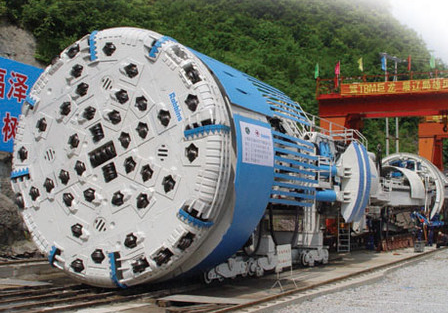
\includegraphics[width=5cm]{figure/TBM.png}
    \end{figure}

\end{columns}

\end{frame}

\subsection[Model]{模型提出}\label{subsec:1-2}
\begin{frame}{模型提出}
\begin{columns}
    \column{.5\textwidth}
        \fs
        {
            \structure{岩体抽样化} \cite{hudson1979discontinuities} 提出岩体的力学行为由岩体裂隙(包括:接缝,裂隙和微裂隙等)的几何参数所决定,而岩体裂隙又可以抽象为扁平的椭球(忽略厚度后可以认为是椭圆)。抽象后的岩体如右图。\\
            在特定采样段,岩体中裂隙的分布就由椭球的九个参数(如下表)满足的概率分布所决定。
        
            \begin{table}[b]
                \centering
                \begin{tabular}{cccc}
                \toprule
                    三个轴长度 & $S_x$ & $S_y$ & $S_z$ \\
                    \midrule
                    三个角度 & $\theta_x$ & $\theta_y$ & $\theta_z$ \\
                    \midrule
                    中心点坐标 & $X$ & $Y$ & $Z$\\ \bottomrule
                \end{tabular}
                \caption{椭球参数表}
                \label{tab:parameters}
            \end{table}
        }
        
    \column{.5\textwidth}
    \begin{figure}
        \centering
        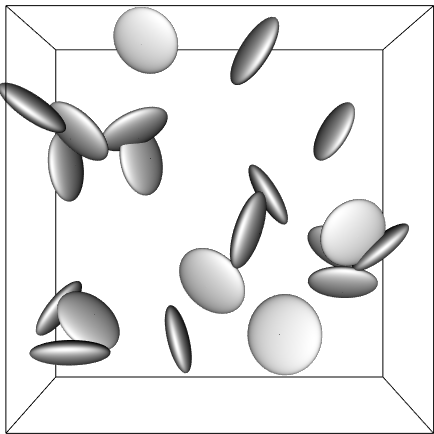
\includegraphics[width=5cm]{figure/abstract.png}
        \caption{岩体抽象}
        \label{fig:abstract}
    \end{figure}
\end{columns}

\end{frame}

\begin{frame}{模型提出}
\fs{
    \alert{基本假设} 假设这九个概率分布独立同分布的,因此可以分开预测,以下仅以参数$S_x$为例。

	\begin{enumerate}
		\item 根据已有时刻$(t = 1, 2, 3, \dots, T)$的椭球样本拟合$S_x$所满足的分布,并且得到每一个时刻分布的参数向量$(\hat{p}_1(1),~ \hat{p}_2(1),~  \dots),$~~ $(\hat{p}_1(2),~ \hat{p}_2(2),~ \dots),$~~ $\dots,$~~ $(\hat{p}_1(T),~ \hat{p}_2(T),~ \dots)$。
		\item 以分布的第一个参数$p_1$为例,它在不同时刻的取值$p_1(t)$构成时间序列。通过的\cite{zhang2003time}所提到的混合ARIMA模型,可以将其拆解为线性部分和非线性部分,即$p_1(t) = L(t) + N(t)$。
		\item 利用第一步所得到的$p_1(t)$的一个抽样${\hat{p}_1(1), \hat{p}_1(2), \dots, \hat{p}_1(T)}$来拟合出$\hat{L}(t)$和$\hat{N}(t)$。
		\item 利用$\hat{L}(t)$和$\hat{N}(t)$得到下一时刻$p_1$的预测值$\hat{L}(T+1)+  \hat{N}(T+1)$。
		\item 重复上述程序可以得到下一个时刻椭球的九个参数所满足的分布以及分布的参数,并且不同时刻椭球的密度${density(1), density(2), \dots, density(t)}$也可看做一个时间序列,利用之前的步骤也就可以得到$T+1$时刻椭圆密度的估计$\hat{d}(T+1)$。
		\item 根据预测得到的九个分布函数和椭圆密度,利用特定的抽样方法,在下一时刻岩体所在的统计窗内抽取裂隙并进行可视化。
	\end{enumerate}
}
\end{frame}
}

\begin{frame}{模型简述}
\fs{
	\alert{问题} 预测TBM近前方椭球的九个参数满足的概率分布函数以及椭球的密度(单位体积椭球中心点的个数)。\\
	\alert{基本假设} 假设这九个概率分布独立同分布的,因此可以分开预测,以下仅以参数$S_x$为例叙述。\\
	\alert{模型简述:}
	\begin{enumerate}
	\item 根据已有时刻$(t = 1, 2, 3, \dots, T)$的椭球样本拟合$S_x$在相应采样段所满足的分布以及分布的参数向量$(\hat{p}_1(T),~ \hat{p}_2(T),~ \dots)$。
	\item 根据分布的参数向量的分量在不同采样段的取值构建和拟合其满足的时间序列模型。
	\item 用前两步中的模型预测TBM近前方$S_x$满足的分布类型和分布的参数向量,以此作为$S_x$的分布函数的预测。
	\end{enumerate}	 
}
\end{frame}